\section{Ход работы}

\subsection{Работа с программой CheckDisk}
\begin{enumerate}
\item
Для запуска программы CheckDisk выполним следующие действия: Пуск -- Мой компьютер -- Правый щелчок по значку диска D -- Свойства -- Сервис -- Выполнить проверку (Рис.~\ref{pic1})
\item
На вкладке Сервис нажмем кнопку ``Выполнить проверку''. В появившемся окне установим необходимые параметры и нажмем ``Начать'' (Рис.~\ref{pic2}). В ряде случаев проверка диска выполнена быть не может, о чем свидетельствует появившееся окно (Рис.~\ref{pic3}) и проверка откладывается до перезагрузки компьютера и выполнится ещё до входа в систему. При нажатии кнопки ``Нет'' появится информационное окно об ошибке (Рис.~\ref{pic4}).
\end{enumerate}

\begin{figure}[h!t] 
  \begin{center}

  \begin{minipage}[h]{0.4\linewidth}
  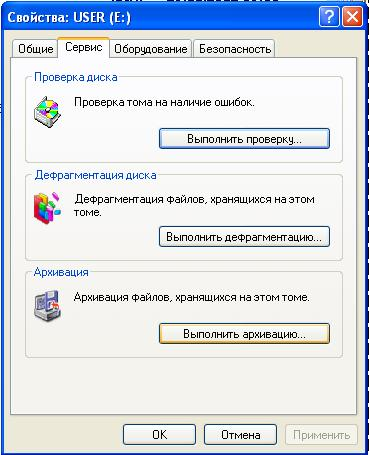
\includegraphics[width=1\linewidth]{1.jpg}
  \caption{\label{pic1}}

  \bigskip
    
  \begin{center}
  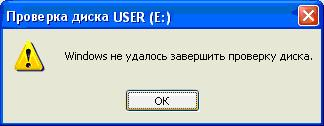
\includegraphics[width=0.8\linewidth]{4.jpg}
  \caption{\label{pic4}}
  \end{center}
  \end{minipage}
  \hfill   
  \begin{minipage}[h]{0.4\linewidth}
  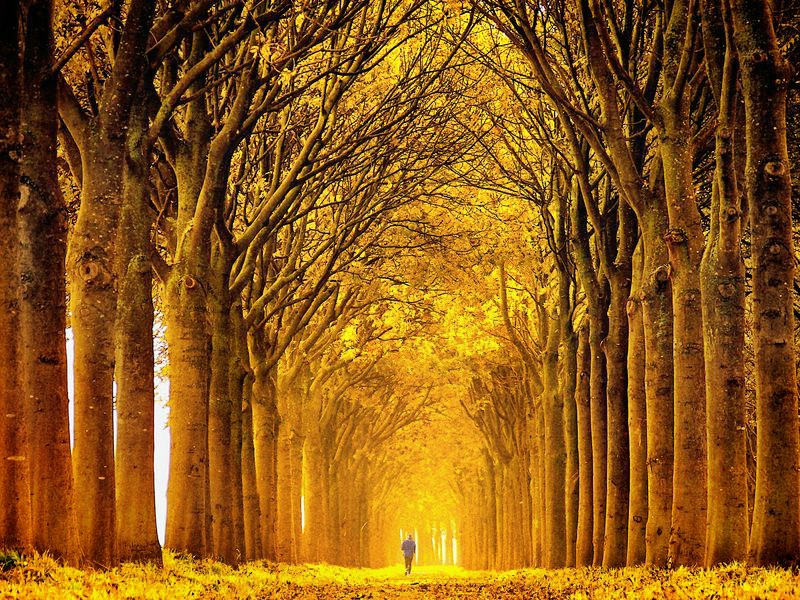
\includegraphics[width=1\linewidth]{3.jpg}
  \caption{\label{pic3}}
  
  \bigskip
  
  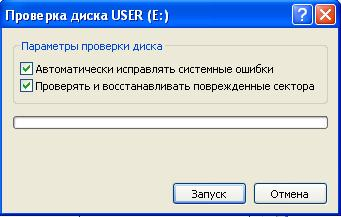
\includegraphics[width=1\linewidth]{2.jpg}
  \caption{\label{pic2}}
  
  \bigskip
    
  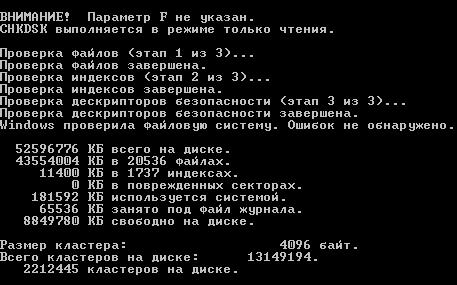
\includegraphics[width=1\linewidth]{5.jpg}
  \caption{\label{pic5}}
  \end{minipage}    
    
  \end{center}
\end{figure}

После проверки появится информационное окно о результатах проверки диска (Рис. ~\ref{pic5}).


\subsection{Работа с программой Disk Defragmenter}

\begin{enumerate}
\item
Для запуска программы дефрагментации диска Disk Defragmenter выполним следующие действия: Пуск -- Программы -- Стандартные -- Служебные -- Дефрагментация диска.
\item
Выбираем необходимый диск, и нажимаем кнопку "Анализ" для определения того, необходима ли этому диску дефрагментация. После завершения анализа окно Дефрагментации выглядит как на Рис. ~\ref{pic6}. В новом диалоговом окне (Рис. ~\ref{pic7}) нажимаем кнопку "Дефрагментация". После проведения этой довольно долгой процедуры система ссобщит об окончании её с помощью информационного окна. Если на диске, нуждающемся в дефрагментации,  менее 15\% свободного дискового пространства система оповестит об этом при помощи диалогового окна (Рис. ~\ref{pic9}).
Произведем анализ тома I: результат представлен на рисунке Рис. ~\ref{pic10}.
\end{enumerate}

\begin{figure}[h!t] 
  \begin{center}

  \begin{minipage}[h]{0.4\linewidth}
  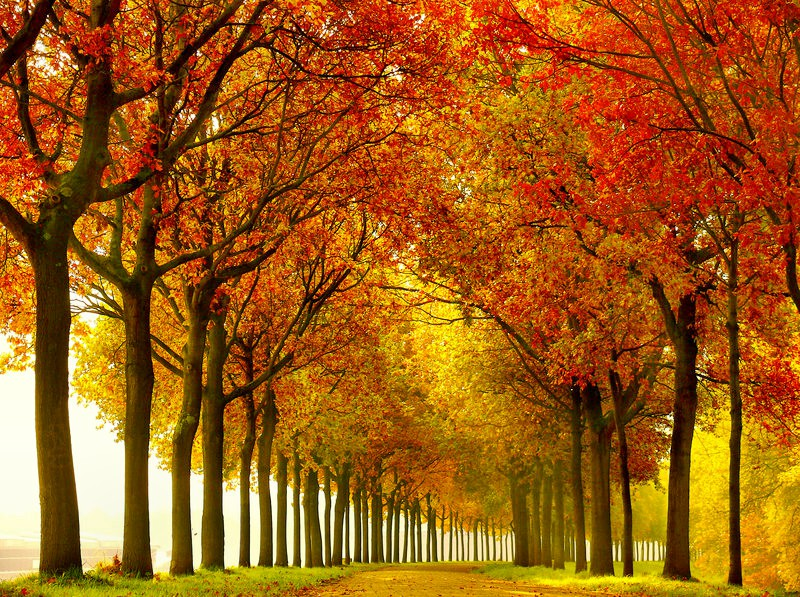
\includegraphics[width=1\linewidth]{6.jpg}
  \caption{\label{pic6}}
  
  \bigskip
  
  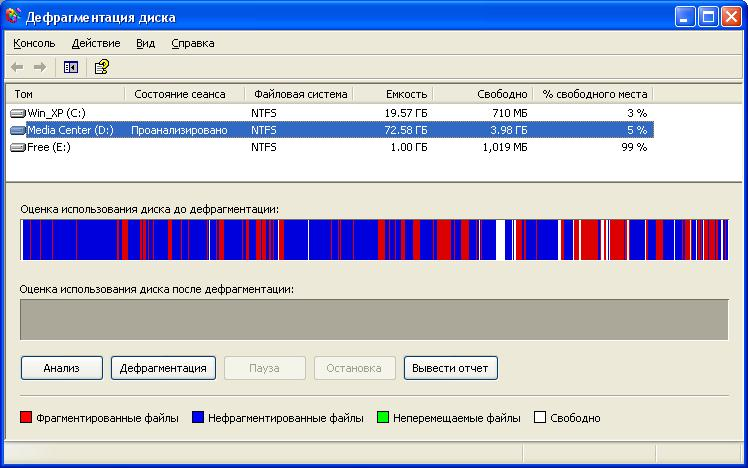
\includegraphics[width=1\linewidth]{7.jpg}
  \caption{\label{pic7}}
  
  \bigskip
  
  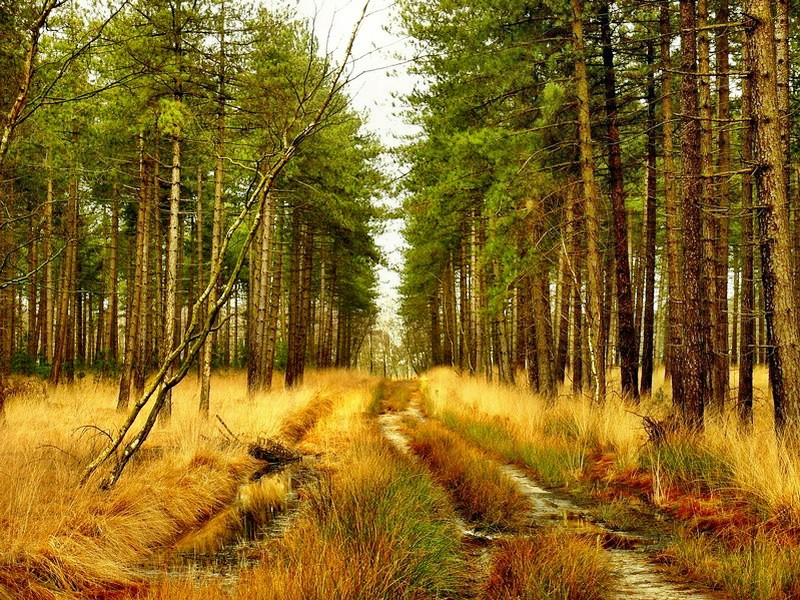
\includegraphics[width=1\linewidth]{8.jpg}
  \caption{\label{pic8}}

  \end{minipage}
  \hfill   
  \begin{minipage}[h]{0.4\linewidth}
  
  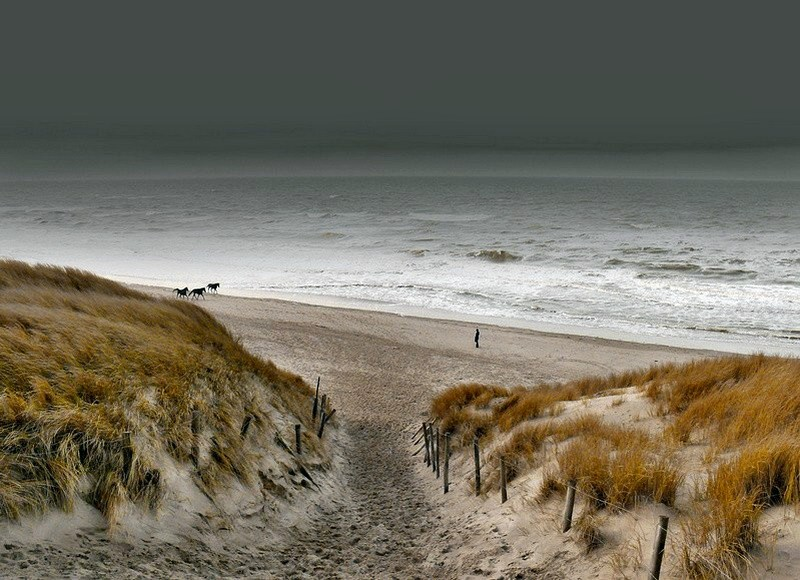
\includegraphics[width=1\linewidth]{10.jpg}
  \caption{\label{pic10}}

  \bigskip
  
  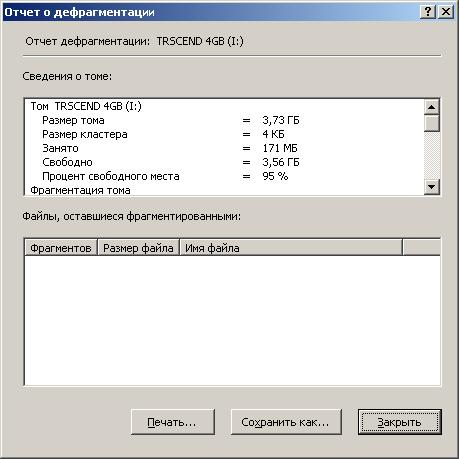
\includegraphics[width=1\linewidth]{11.jpg}
  \caption{\label{pic11}}

  \end{minipage}    
  \begin{minipage}[h]{1\linewidth}	        
 
  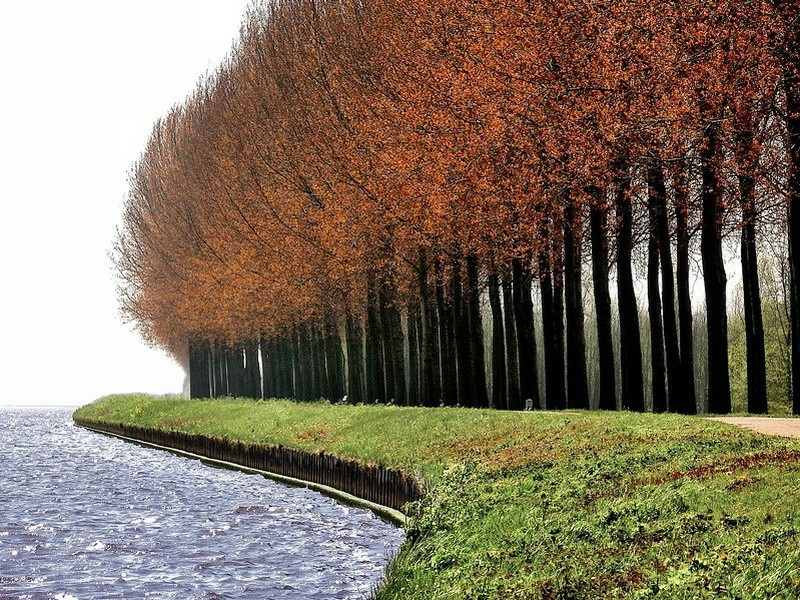
\includegraphics[width=1\linewidth]{9.jpg}
  \caption{\label{pic9}}
  
  \end{minipage}        
  \end{center}
\end{figure}


В конце дефрагментации выведем отчёт (кнопка Вывести отчет) о результатах дефрагментации (риc. ~\ref{pic11}).

\subsection{Сжатие файлов и папок}

\begin{enumerate}
\item
  Создадим на FAT-диске (в нашем случае это флеш-диск) непустую папку, вызовем контекстное меню правым кликом по этой папке, выберем меню Отправить -- Сжатая ZIP-папка (рис. ~\ref{pic12}).
\item
  Создадим непустую папку на NTFS-диске (в нашем случае это диск D:), вызовем контекстное меню правым кликом по этой папке, выберем Свойства -- Общие -- Другие и выставим флажок ``Сжимать диск для экономии места'', нажмем ОК и Применить (рис. ~\ref{pic13}).

\end{enumerate}

\begin{figure}[h!t] 
  \begin{center}

  \begin{minipage}[h]{0.4\linewidth}

  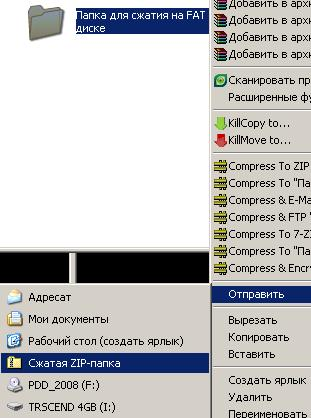
\includegraphics[width=1\linewidth]{12.jpg}
  \caption{\label{pic12}}

  \end{minipage}
  \hfill   
  \begin{minipage}[h]{0.4\linewidth}
  
  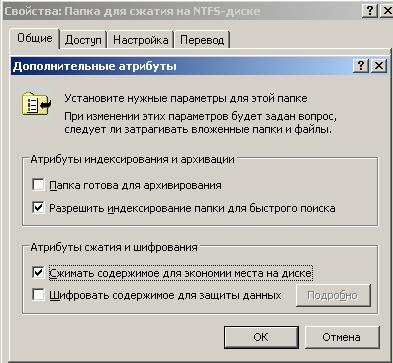
\includegraphics[width=1\linewidth]{13.jpg}
  \caption{\label{pic13}}

  \end{minipage}          
  \end{center}
\end{figure}


\subsection{Команды Windows для работы с файловыми системами и дисками}
\begin{enumerate}
\item
Воспользуемся командой subst -- сопоставление имени виртуального диска указанному пути. Введем команду subst как требует шаблон. Сопоставим виртуальному диску М: папку DST на физическом диске D: (рис. ~\ref{pic14})

\begin{figure}[h!t] 
  \begin{center}

  \begin{minipage}[h]{0.4\linewidth}

  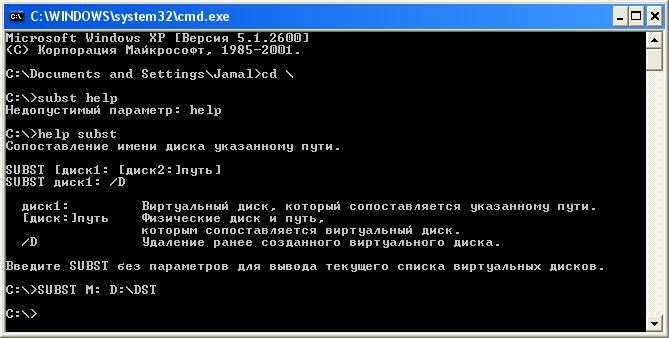
\includegraphics[width=1\linewidth]{14.jpg}
  \caption{\label{pic14}}

  \end{minipage}
  \hfill   
  \begin{minipage}[h]{0.4\linewidth}
  
  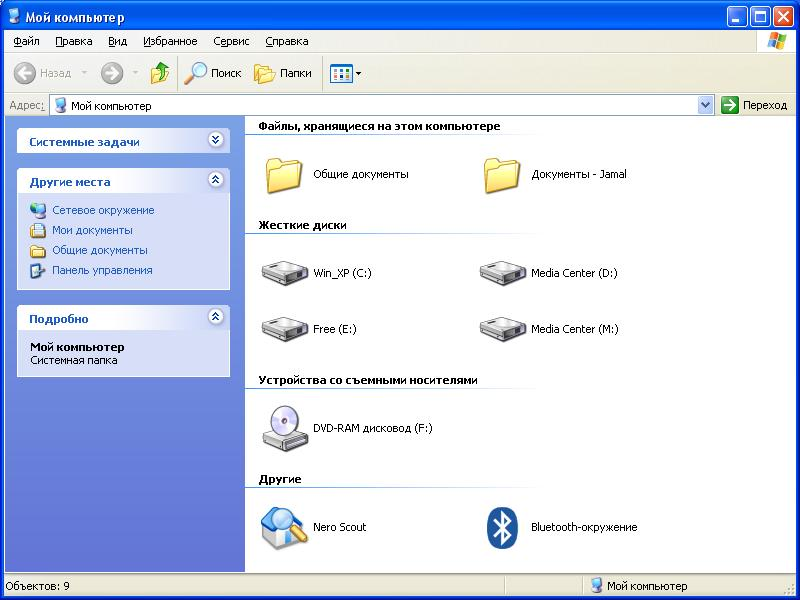
\includegraphics[width=1\linewidth]{15.jpg}
  \caption{\label{pic15}}

  \end{minipage}          
  \end{center}
\end{figure}


На рис. ~\ref{pic15} мы видим ,что появился том М:, соответствующий папке DST.

\end{enumerate}


\subsection{Архивация данных программой NTBackup}

\begin{enumerate}

\item
  Создадим, как и требовалось на диске Е: папку А, в ней папку В, а также скопируем туда папку ``Мои документы'', в папку В скопируем произвольно выбранную папку. Структура папок видна на риc. ~\ref{pic16}.
\item
  Cоздадим полный архив папки А с помощью NTBackup. Для запуска программы архивации выберем Пуск -- Программы -- Стандартные -- Служебные -- Архивация данных. Объем папки А равен 59 744 357 байт. Процесс подготовки и архивации изображен на рис. ~\ref{pic17} -- ~\ref{pic24}.

\begin{figure}[h!t] 
  \begin{center}

  \begin{minipage}[h]{0.4\linewidth}

  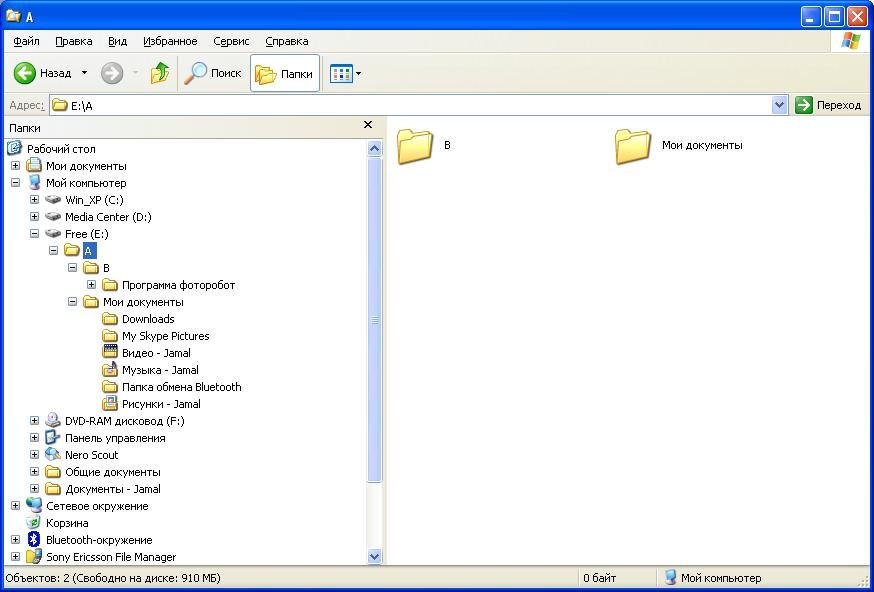
\includegraphics[width=1\linewidth]{16.jpg}
  \caption{\label{pic16}}

  \bigskip
  
  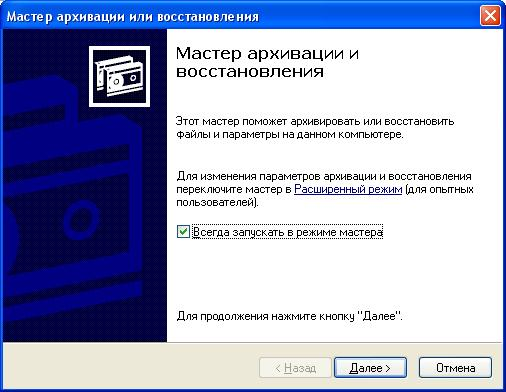
\includegraphics[width=1\linewidth]{17.jpg}
  \caption{\label{pic17}}

  \bigskip
    
  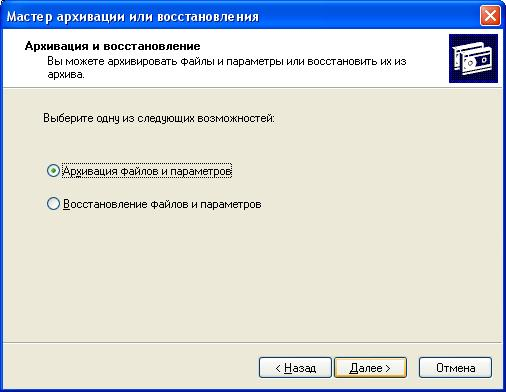
\includegraphics[width=1\linewidth]{18.jpg}
  \caption{\label{pic18}}

  \bigskip
  
  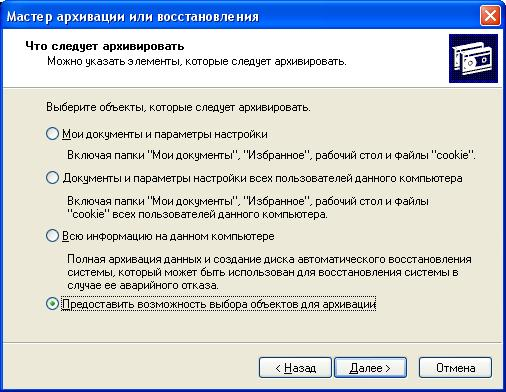
\includegraphics[width=1\linewidth]{19.jpg}
  \caption{\label{pic19}}
  
  \end{minipage}
  \hfill   
  \begin{minipage}[h]{0.4\linewidth}

  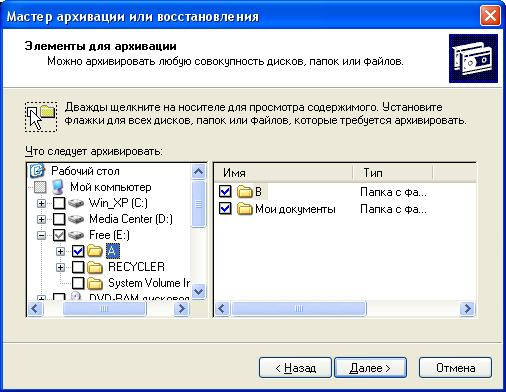
\includegraphics[width=1\linewidth]{20.jpg}
  \caption{\label{pic20}}

  \bigskip
      
  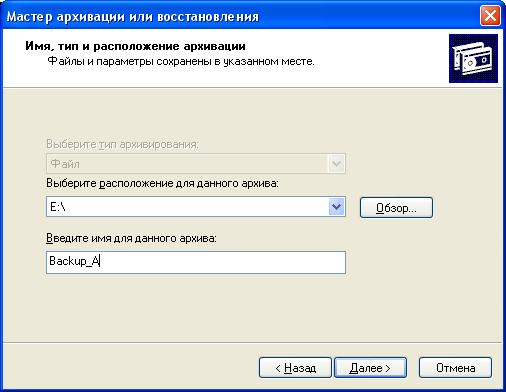
\includegraphics[width=1\linewidth]{21.jpg}
  \caption{\label{pic21}}

  \bigskip
  
  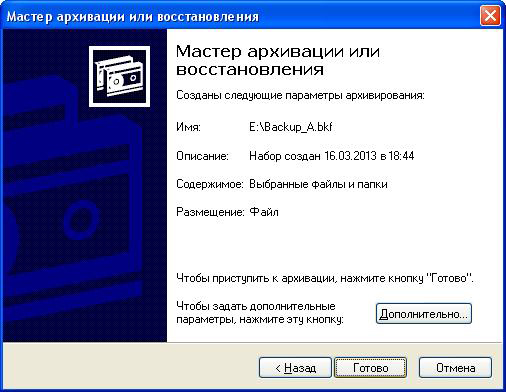
\includegraphics[width=1\linewidth]{22.jpg}
  \caption{\label{pic22}}

  \end{minipage}          
  \end{center}
\end{figure}

\begin{figure}[h!t] 
  \begin{center}
  \begin{minipage}[h]{0.4\linewidth}
  
  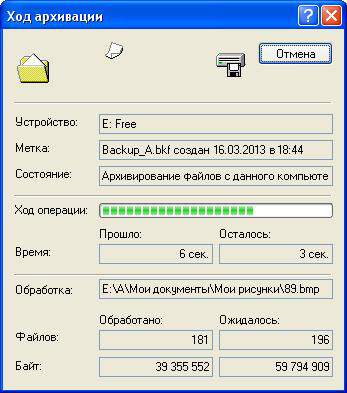
\includegraphics[width=1\linewidth]{23.jpg}
  \caption{\label{pic23}}

  \bigskip
 
  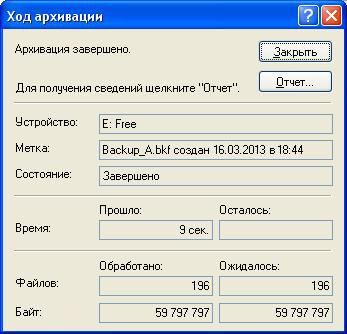
\includegraphics[width=1\linewidth]{24.jpg}
  \caption{\label{pic24}}

  \bigskip
    
  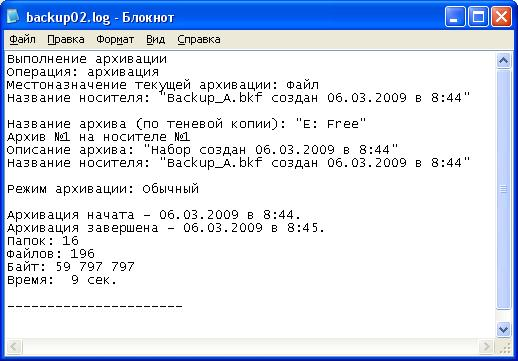
\includegraphics[width=1\linewidth]{25.jpg}
  \caption{\label{pic25}}

  \bigskip
      
  \end{minipage}
  \hfill   
  \begin{minipage}[h!]{0.4\linewidth}

  \bigskip
    
  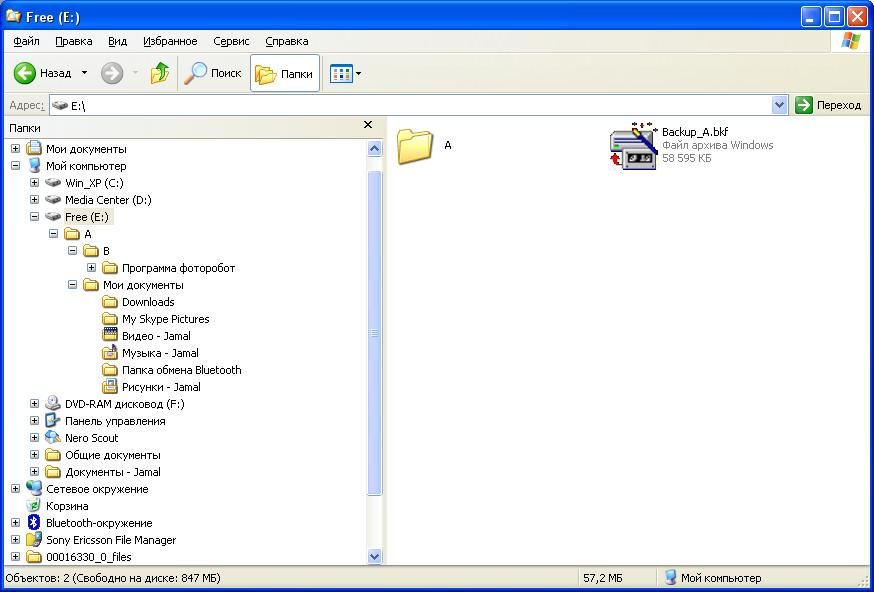
\includegraphics[width=1\linewidth]{26.jpg}
  \caption{\label{pic26}}

  \bigskip
    
  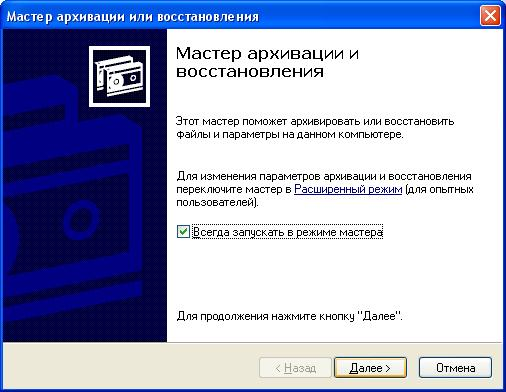
\includegraphics[width=1\linewidth]{27.jpg}
  \caption{\label{pic27}}

  \bigskip
    
  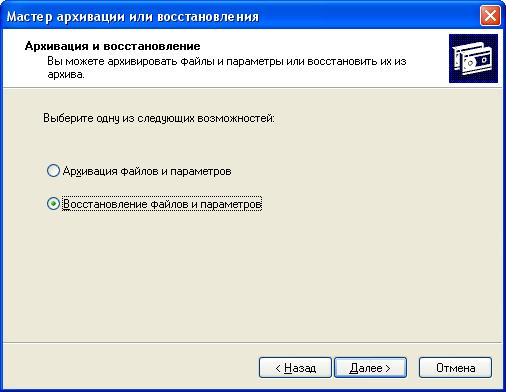
\includegraphics[width=1\linewidth]{28.jpg}
  \caption{\label{pic28}}
    
  \end{minipage}          
  \end{center}
\end{figure}



Файл с архивными данными появился в указанном месте (рис. ~\ref{pic26}). Объем резервной копии равен 60 001 280 байт.

\item
  Удалим нашу папку А и восстановим ее. Для этого нажмем кнопки Мастер восстановления -- Далее щёлкнем по символу ``+'' для отображения файла резервной копии выберем устройство в поле со списком Выбор архива, установим флажки напротив соответствующих полей для папок и файлов, которые мы хотите восстановить; выберем соответствующие опции и нажжем по кнопке Готово. Ход восстановления представлен на рис. ~\ref{pic27} -- ~\ref{pic33}.

\begin{figure}[h!t] 
  \begin{center}
  \begin{minipage}[h]{0.4\linewidth}

  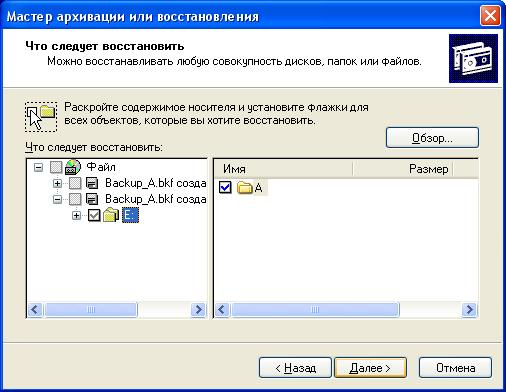
\includegraphics[width=1\linewidth]{29.jpg}
  \caption{\label{pic29}}  

  \bigskip
  
  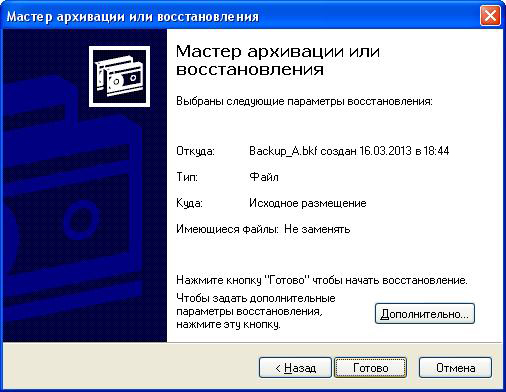
\includegraphics[width=1\linewidth]{30.jpg}
  \caption{\label{pic30}}

  \bigskip
  
  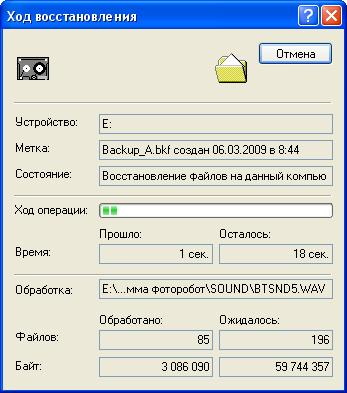
\includegraphics[width=1\linewidth]{31.jpg}
  \caption{\label{pic31}}  

  \bigskip
    
  \end{minipage}
  \hfill   
  \begin{minipage}[h]{0.4\linewidth}

  \bigskip
    
  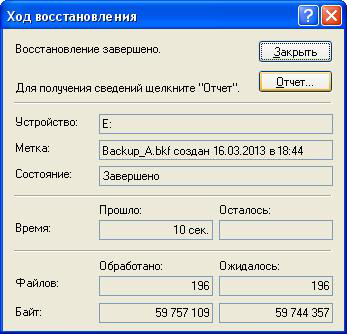
\includegraphics[width=1\linewidth]{32.jpg}
  \caption{\label{pic32}}
  
  \bigskip

  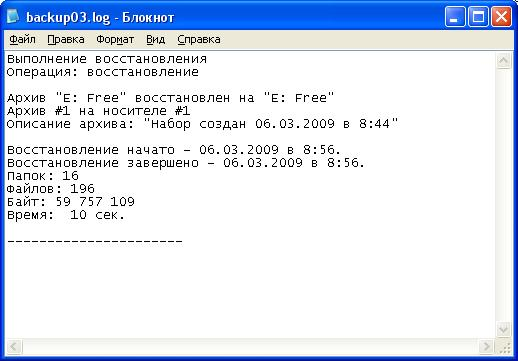
\includegraphics[width=1\linewidth]{33.jpg}
  \caption{\label{pic33}}
  
  \bigskip
  
  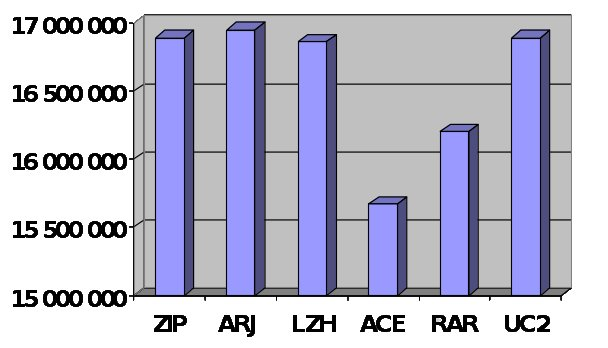
\includegraphics[width=1\linewidth]{34.jpg}
  \caption{\label{pic34}}

  \end{minipage}          
  \end{center}
\end{figure}

\end{enumerate}

\subsection{Работа с архиваторами}

\begin{enumerate}
\item
  Работа с архиваторами ZIP, ARJ, LHA, RAR, UC2 и ACE представлена в таблице ~\ref{tab1}. Архивируем папку А.


\begin{table}[h!tbp]
  \caption{\label{tab1}}
  \begin{tabular}{| p{2cm} | p{2cm} | p{2cm} | p{2cm} | p{2cm} | p{2cm} | p{2cm}l |}
    \hline
    & \multicolumn{6}{c}{Архиватор} &  \\ \cline{2-8}
    &\centering ZIP &\centering ARJ &\centering LZH &\centering ACE &\centering RAR &\centering UC2 & \\
    \hline
    \centering Размер файла в байтах &\centering 16 889 887 &\centering 16 947 410 &\centering 16 859 863 &\centering 15 671 986 &\centering 16 200 997 &\centering 16 889 887 & \\ 
    \hline
  \end{tabular}
\end{table}


\item
  Результаты архивирования схематически представлены на рис. ~\ref{pic34}. По результатам архивирования можно сделать вывод, что эффективность использовавшихся архиваторов находится в среднем на одном уровне.

\end{enumerate}
\clearpage
